% Problem Set -- an A4 homework sheet in Libertinus with a dark rust accent.
% Edit the course details in the "Course details" block below, then write
% problems with \begin{problem}{points}{title} ... \end{problem}.

% ---- The one switch -------------------------------------------------------
% \showsolutionstrue prints every solution box; \showsolutionsfalse hands out
% the blank sheet. It sits before \documentclass so it is the first thing seen.
\newif\ifshowsolutions
\showsolutionstrue

\documentclass[11pt,a4paper]{article}

% ---- Page ----------------------------------------------------------------
% A wide left margin holds the point badges; the measure stays near 75
% characters, comfortable for prose mixed with display maths.
\usepackage[a4paper,top=20mm,bottom=22mm,left=40mm,right=28mm,
            marginparwidth=24mm,marginparsep=5mm,headsep=9mm]{geometry}

% ---- Fonts ---------------------------------------------------------------
% Libertinus Serif for text, its matching maths via libertinust1math.
\usepackage[T1]{fontenc}
\usepackage{libertinus-type1}
\usepackage[scaled=0.97]{libertinust1math}
\usepackage{amsmath}
\usepackage[final]{microtype}

% ---- Colour: change the accent here --------------------------------------
\usepackage{xcolor}
\definecolor{rust}{HTML}{8A3A16}     % dark rust accent
\colorlet{rustpale}{rust!6!white}    % solution background
\colorlet{rule}{rust!45!white}       % hairlines
\colorlet{ink}{black!82}

% ---- Tools ---------------------------------------------------------------
\usepackage{booktabs,tabularx,array}
\usepackage{enumitem}
\usepackage{tikz}
\usetikzlibrary{positioning}
\usepackage[most]{tcolorbox}
\usepackage{fancyhdr,lastpage}
\usepackage[hidelinks]{hyperref}

\setlength{\parindent}{0pt}
\setlength{\parskip}{0.45\baselineskip}
\frenchspacing
\widowpenalty=10000 \clubpenalty=10000

% ---- Course details: edit these ------------------------------------------
\newcommand{\coursecode}{MATH 2410}
\newcommand{\coursename}{Probability Theory}
\newcommand{\term}{Autumn 2026}
\newcommand{\assignment}{4}
\newcommand{\assignmenttopic}{Conditioning, Densities and Expectation}
\newcommand{\duedate}{Friday 30 October, 17:00}
\newcommand{\instructor}{Dr.\ Imogen Hale}

% ---- Running head and foot -----------------------------------------------
\pagestyle{fancy}
\fancyhf{}
\renewcommand{\headrulewidth}{0pt}
\fancyhead[L]{\footnotesize\color{rust}\textsc{\MakeLowercase{\coursecode}} \textperiodcentered{} \textsc{problem set \assignment}}
\fancyhead[R]{\footnotesize\color{black!55}\ifshowsolutions\textsc{with solutions}\fi}
\fancyfoot[C]{\footnotesize\color{black!55}\thepage\ of \pageref{LastPage}}
\fancypagestyle{first}{\fancyhf{}\fancyfoot[C]{\footnotesize\color{black!55}\thepage\ of \pageref{LastPage}}}

% ---- Header fields --------------------------------------------------------
% A labelled blank line for name and ID; \fieldline sets the label in small
% caps over a hairline so the handwritten entry has a place to sit.
\newcommand{\fieldline}[2]{%
  \begin{minipage}[b]{#2}
    \vspace{6mm}{\color{rule}\hrule height 0.4pt}\vspace{1.2mm}
    {\scriptsize\color{rust}\textsc{\MakeLowercase{#1}}}
  \end{minipage}}

% ---- Points table -----------------------------------------------------------
% Each problem writes its points to the aux file; the table at the top reads
% them back on the next run, so its rows and total follow the problems.
% latexmk reruns until they settle.
\makeatletter
\newcount\ps@total
\def\ps@rows{}
\newcommand{\pointsentry}[2]{%
  \g@addto@macro\ps@rows{#1 & #2 & \\}\global\advance\ps@total#2\relax}
\newcommand{\recordpoints}[1]{%
  \protected@write\@auxout{}{\string\pointsentry{\theproblem}{#1}}}
\newcommand{\pointsrows}{\ps@rows}
\newcommand{\pointstotal}{\the\ps@total}
\makeatother

% ---- Problems -------------------------------------------------------------
% \begin{problem}{points}{title}: the number and title open the problem, the
% point badge hangs in the left margin, aligned to the heading's baseline.
\newcounter{problem}
\newcommand{\pointbadge}[1]{%
  \llap{\tikz[baseline=(b.base)]\node[draw=rust,line width=0.5pt,
    rounded corners=2pt,inner xsep=3pt,inner ysep=1.6pt,text=rust,
    font=\sffamily\scriptsize] (b) {#1\,pts};\hspace{6mm}}}
\newenvironment{problem}[2]{%
  \refstepcounter{problem}%
  \recordpoints{#1}%
  \par\addvspace{1.2\baselineskip}\penalty-200
  % The statement and its parts never split across pages.
  \noindent\begin{minipage}{\linewidth}\setlength{\parskip}{0.45\baselineskip}%
  \leavevmode\pointbadge{#1}%
  {\color{rust}\large\textsc{problem}~\theproblem}%
  \hspace{0.6em}{\color{rule}\textbar}\hspace{0.6em}%
  {\itshape #2}\par\vspace{0.2\baselineskip}%
}{\end{minipage}\par}

% Sub-parts (a), (b), (c) hang their labels in the gutter of the text.
\setlist[enumerate,1]{label=\textup{(\alph*)},leftmargin=2em,labelsep=0.6em,
  itemsep=0.3\baselineskip,topsep=0.2\baselineskip}

% ---- Solutions ------------------------------------------------------------
% A pale rust panel with a rust spine on the left; breakable so long proofs
% continue across pages. With \showsolutionsfalse the body is discarded.
\newtcolorbox{solutionbox}{enhanced,breakable,colback=rustpale,
  colframe=rustpale,boxrule=0pt,arc=0pt,left=10pt,right=10pt,top=6pt,
  bottom=6pt,before skip=0.6\baselineskip,after skip=0.4\baselineskip,
  borderline west={1.2pt}{0pt}{rust},
  fontupper=\color{ink},
  % tcolorbox resets \parskip; restore it so solution paragraphs breathe.
  before upper={\setlength{\parskip}{0.4\baselineskip}}}
\ifshowsolutions
  \NewDocumentEnvironment{solution}{+b}
    {\begin{solutionbox}{\small\color{rust}\textsc{solution}}\par\vspace{0.2\baselineskip}#1\end{solutionbox}}{}
\else
  \NewDocumentEnvironment{solution}{+b}{}{}
\fi

\newcommand{\Prob}{\mathbb{P}}
\newcommand{\E}{\mathbb{E}}
\newcommand{\Var}{\operatorname{Var}}
\newcommand{\dd}{\,\mathrm{d}}

\begin{document}
\thispagestyle{first}

% ---- Title block -----------------------------------------------------------
\begin{minipage}[t]{0.58\textwidth}
  {\small\color{rust}\textsc{\MakeLowercase{\coursecode}} \textperiodcentered{} \textsc{\MakeLowercase{\coursename}} \textperiodcentered{} \textsc{\MakeLowercase{\term}}}\par
  \vspace{3mm}
  {\fontsize{26}{28}\selectfont Problem Set \assignment}\par
  \vspace{1.5mm}
  {\itshape\color{ink}\assignmenttopic}\par
  \vspace{3mm}
  {\small Due \textbf{\duedate} \textperiodcentered{} \instructor}
\end{minipage}%
\hfill
\begin{minipage}[t]{0.34\textwidth}
  \vspace{0pt}\small
  % Points table: rows and total come from the problems; the score column
  % is left blank for the grader.
  \begin{tabular*}{\linewidth}{@{\extracolsep{\fill}}l c c@{}}
    \toprule
    \textsc{problem} & \textsc{points} & \textsc{score} \\
    \midrule
    \pointsrows
    \midrule
    \textsc{total} & \pointstotal & \\
    \bottomrule
  \end{tabular*}
\end{minipage}

\vspace{2mm}
\fieldline{Student name}{0.62\textwidth}\hfill\fieldline{Student ID}{0.30\textwidth}

\vspace{4mm}
{\color{rust}\hrule height 0.6pt}
\vspace{2.5mm}
{\small\itshape Show your reasoning: a correct number without justification earns
at most half the points. Collaboration is welcome, but write up your own
solutions and name the people you worked with.}
\vspace{1mm}

% ---- Problem 1 ---------------------------------------------------------------
\begin{problem}{10}{A screening test}
A blood test for a condition that affects $2\%$ of a population detects it in
$95\%$ of people who have it (sensitivity) and correctly clears $90\%$ of
people who do not (specificity). A person is drawn at random and tested.
\begin{enumerate}
  \item Draw the probability tree for condition and test result.
  \item Find the probability that the test is positive.
  \item Given a positive result, how likely is it that the person has the
        condition? Comment on the size of your answer.
\end{enumerate}
\end{problem}

\begin{solution}
(a) Let $D$ be the event that the person has the condition and $T$ that the
test is positive. The tree branches first on $D$, then on $T$:

\begin{center}
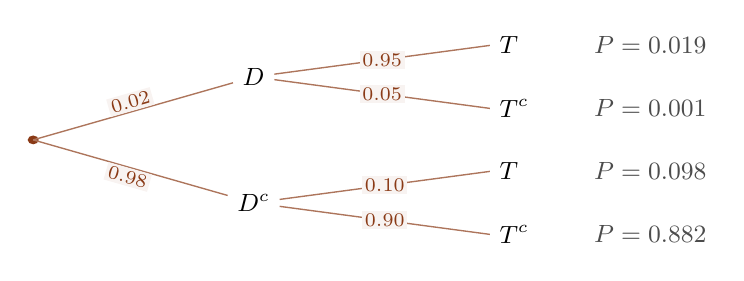
\begin{tikzpicture}[font=\small,x=1mm,y=0.8mm,
    br/.style={draw=rust!70,line width=0.5pt},
    pr/.style={font=\scriptsize,color=rust,fill=rustpale,inner sep=1pt}]
  % Root, first split on the condition, second split on the test result.
  \fill[rust] (0,0) circle (0.7);
  \node (D)  at (28, 10) {$D$};
  \node (Dc) at (28,-10) {$D^c$};
  \draw[br] (0,0) -- node[pr,above,sloped] {$0.02$} (D);
  \draw[br] (0,0) -- node[pr,below,sloped] {$0.98$} (Dc);
  \foreach \from/\y/\lab/\p/\joint in {D/15/T/0.95/0.019, D/5/T^c/0.05/0.001,
      Dc/-5/T/0.10/0.098, Dc/-15/T^c/0.90/0.882} {
    \node[anchor=west] (leaf) at (58,\y) {$\lab$};
    \draw[br] (\from) -- node[pr,midway] {$\p$} (leaf.west);
    \node[anchor=west,color=black!70] at (70,\y) {$\Prob = \joint$};
  }
\end{tikzpicture}
\end{center}

(b) By the law of total probability, summing the two leaves that end in $T$,
\begin{align*}
  \Prob(T) &= \Prob(T\mid D)\,\Prob(D) + \Prob(T\mid D^c)\,\Prob(D^c) \\
           &= 0.95\cdot0.02 + 0.10\cdot0.98 = 0.019 + 0.098 = 0.117.
\end{align*}

(c) Bayes' rule gives
\begin{equation*}
  \Prob(D\mid T) = \frac{\Prob(T\mid D)\,\Prob(D)}{\Prob(T)}
                 = \frac{0.019}{0.117} \approx 0.162.
\end{equation*}
Only about one positive in six is a true case. The condition is rare, so the
$10\%$ false-positive rate among the healthy $98\%$ produces five times more
positives than the sick $2\%$ do.
\end{solution}

% ---- Problem 2 ---------------------------------------------------------------
\begin{problem}{12}{A polynomial density}
A random variable $X$ has density $f(x) = c\,x^2$ for $0 \le x \le 2$ and
$f(x)=0$ elsewhere.
\begin{enumerate}
  \item Find the constant $c$.
  \item Find the distribution function $F(x)$ and use it to compute
        $\Prob(X > 1)$.
  \item Compute $\E[X]$ and $\Var(X)$.
\end{enumerate}
\end{problem}

\begin{solution}
(a) The density must integrate to one:
$\int_0^2 c\,x^2\dd x = \tfrac{8c}{3} = 1$, so $c = \tfrac38$.

(b) For $0\le x\le 2$, $F(x) = \int_0^x \tfrac38 t^2\dd t = x^3/8$, with
$F(x)=0$ for $x<0$ and $F(x)=1$ for $x>2$. Hence
$\Prob(X>1) = 1 - F(1) = \tfrac78$.

(c) The first two moments are
\begin{align*}
  \E[X]   &= \int_0^2 x\cdot\frac38 x^2\dd x = \frac38\cdot\frac{2^4}{4} = \frac32, \\
  \E[X^2] &= \int_0^2 x^2\cdot\frac38 x^2\dd x = \frac38\cdot\frac{2^5}{5} = \frac{12}{5},
\end{align*}
so that
\begin{equation*}
  \Var(X) = \E[X^2] - \E[X]^2 = \frac{12}{5} - \frac94 = \frac{3}{20}.
\end{equation*}
The mean lies right of the midpoint $1$, as expected for a density that
grows with $x$.
\end{solution}

% ---- Problem 3 ---------------------------------------------------------------
\begin{problem}{10}{Waiting for a success}
A basketball player makes each free throw independently with probability
$p\in(0,1)$. Let $N$ be the number of throws up to and including the first
success.
\begin{enumerate}
  \item Show that $\Prob(N>n) = (1-p)^n$ for $n = 0,1,2,\dots$
  \item Prove the memoryless property
        $\Prob(N > m+n \mid N > m) = \Prob(N > n)$.
  \item Use $\E[N] = \sum_{n\ge0}\Prob(N>n)$ to find $\E[N]$.
\end{enumerate}
\end{problem}

\begin{solution}
(a) The event $\{N>n\}$ happens exactly when the first $n$ throws all miss.
By independence its probability is $(1-p)^n$.

(b) Because $\{N>m+n\}\subseteq\{N>m\}$, the intersection of the two events is
the smaller one, and
% The shallow last row leaves amsmath's strut below the ink; a shorter skip
% gives the same visible gap as the displays that end on a fraction.
{\setlength{\belowdisplayskip}{8.6pt plus 3pt minus 6pt}%
\begin{align*}
  \Prob(N > m+n \mid N > m) &= \frac{\Prob(N>m+n)}{\Prob(N>m)}
     = \frac{(1-p)^{m+n}}{(1-p)^m} \\
  &= (1-p)^n = \Prob(N>n),
\end{align*}}%
so past misses say nothing about the wait still to come.

(c) Summing the geometric series,
\begin{equation*}
  \E[N] = \sum_{n\ge0}(1-p)^n = \frac{1}{1-(1-p)} = \frac1p .
\end{equation*}
A player who scores $80\%$ of the time waits $1.25$ throws on average.
\end{solution}

% ---- Problem 4 ---------------------------------------------------------------
\begin{problem}{8}{Returned coats}
At the end of a concert, an attendant hands $n$ coats back to their $n$ owners
in uniformly random order. Let $M$ be the number of people who receive their
own coat.
\begin{enumerate}
  \item Write $M$ as a sum of indicator variables and find $\E[M]$.
  \item Find $\Var(M)$.
\end{enumerate}
\end{problem}

\begin{solution}
(a) Let $I_k = 1$ if person $k$ gets their own coat and $0$ otherwise, so
$M = I_1+\dots+I_n$. Each person is equally likely to get any of the $n$ coats,
so $\E[I_k] = 1/n$, and linearity of expectation gives
$\E[M] = n\cdot\tfrac1n = 1$, whatever the size of the audience.

(b) For $j\ne k$, $\E[I_jI_k] = \frac{1}{n}\cdot\frac{1}{n-1}$, the chance
that both get their coats. Since $I_k^2 = I_k$,
\begin{align*}
  \E[M^2] &= \sum_k \E[I_k] + \sum_{j\ne k}\E[I_jI_k]
           = 1 + n(n-1)\cdot\frac{1}{n(n-1)} = 2, \\
  \Var(M) &= \E[M^2] - \E[M]^2 = 2 - 1 = 1.
\end{align*}
Mean and variance both equal one, a first hint that $M$ is close to a
Poisson$(1)$ variable when $n$ is large.
\end{solution}

% ---- Problem 5 ---------------------------------------------------------------
\begin{problem}{10}{Two dice, two summaries}
Roll two fair dice. Let $X$ be the smaller and $Y$ the larger of the two
faces, so that $X \le Y$ always.
\begin{enumerate}
  \item Find $\Prob(X = j,\,Y = k)$ for $j \le k$, and then $\Prob(X = k)$.
  \item Find $\E[X]$, and deduce $\E[Y]$ without further sums.
  \item Are $X$ and $Y$ independent? Justify in one line.
\end{enumerate}
\end{problem}

\begin{solution}
(a) The outcome $(X,Y)=(j,k)$ with $j<k$ arises from two ordered rolls,
$(j,k)$ and $(k,j)$, while $j=k$ arises from one, so $\Prob(X=j,Y=k)$ is $2/36$ or $1/36$.
Summing over the $6-k$ larger values of $Y$,
\begin{equation*}
  \Prob(X = k) = \frac{1 + 2(6-k)}{36} = \frac{13-2k}{36},
  \qquad k = 1,\dots,6.
\end{equation*}

(b) Using $\sum_{k=1}^6 k = 21$ and $\sum_{k=1}^6 k^2 = 91$,
\begin{equation*}
  \E[X] = \sum_{k=1}^{6} k\,\frac{13-2k}{36}
        = \frac{13\cdot21 - 2\cdot91}{36} = \frac{91}{36} \approx 2.53.
\end{equation*}
Since $X+Y$ is the sum of the two faces, $\E[X]+\E[Y] = 7$, so
$\E[Y] = 7 - \frac{91}{36} = \frac{161}{36} \approx 4.47$.

(c) No: $\Prob(X=2,\,Y=1) = 0$, but $\Prob(X=2)\,\Prob(Y=1) > 0$.
\end{solution}

\end{document}
